\chapter{zad5}
Zadanie 5 polegało na dobraniu nastaw regulatora PID i DMC metodą eksperymentalną w oparciu o przebiegi i wskaźnik jakości regulacji $E$:

\begin{equation}
    E = \sum_{k=1}^{k_{\mathrm{konc}}}(y^{\mathrm{zad}}(k)-y(k))^{2}
\end{equation}

dla zaproponowanej przez nas trajektorii zmian sygnału zadanego $y^{\mathrm{zad}}$ (Rys 6.1.).

\begin{figure}[tb] 
\centering 
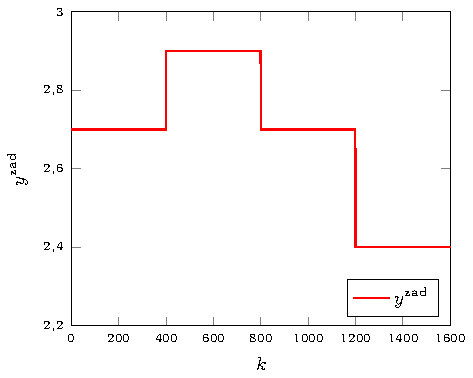
\includegraphics[scale=1]{rysunki/zapisz_pdf/y_zad.pdf} 
\caption{Trajektoria zmian sygnału $y^{\mathrm{zad}}$ na której przeprowadzimy symulacje} 
\label{r_pgfplots_trajektoria} 
\end{figure}

Ponieważ wskaźnik $E$ zliczany był już w poprzednim zadaniu, kod Matlabowy będzie tu taki sam jak w zadaniu 4.

\section{Eksperymentalne dobranie parametrów PID}
Do eksperymentalnego dobrania parametrów PID użyto nastepującej metody eksperymentalnej:
\begin{enumerate}
\item Zwiekszanie wpływu członu P przy wyłączonych członach I i D, aż dla pojedyńczego skoku wartości zadanej, wartość regulowana będzie wykonywała stałe, niegasnące oscylacje wokół wartości zadanej.
\item Dla wartości równej połowie uzyskanej w kroku pierwszym i wyłączonym członie D, dobranie wartości $T_{\mathrm{i}}$ dającej zadowalające wyniki.
\item Dla wartości $K$ i $T_{\mathrm{i}}$ dobranych w kroku drugim, dobranie wartości $T_{\mathrm{d}}$ dającej zadowalające wyniki.
\end{enumerate}


Stałe oscylacje obiektu osiągnięto dla $K_{\mathrm{kryt}}=\num{3.95}$ (Rys 6.2.).


\begin{figure}[tb] 
\centering 
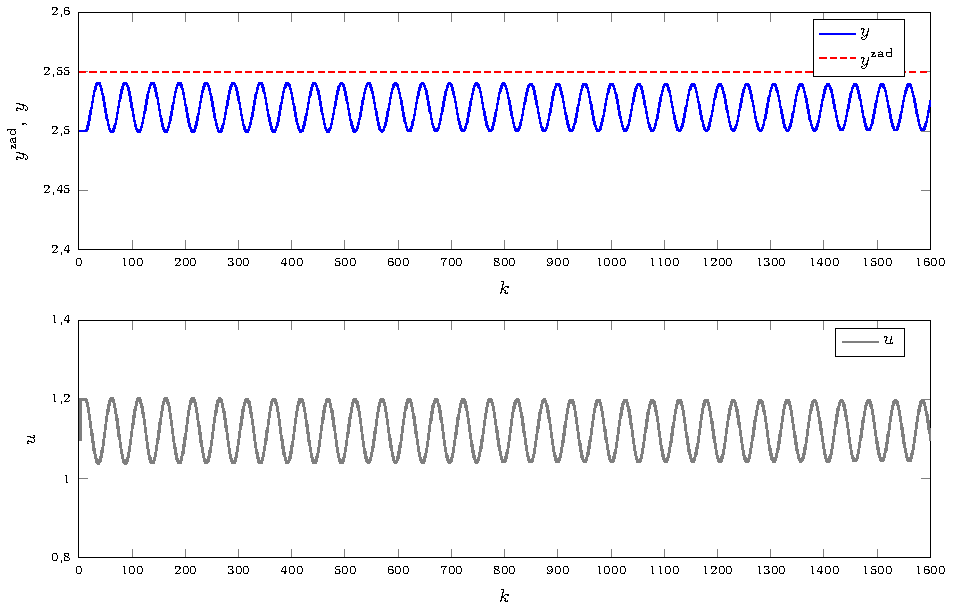
\includegraphics[scale=1]{rysunki/zapisz_pdf/oscylacje.pdf} 
\caption{Stałe (w pewnym przybliżeniu) oscylacje wartości wyjściowej $y$} 
\label{r_pgfplots_funkcje} 
\end{figure}


Warto zaznaczyć, że z powodu ograniczeń, każda wartość oscylacji powodująca ich rośnięcie doprowadzi w końcu do stałych oscylacji - należy więc być ostrożnym z dobieraniem parametru K, żeby parametr u nie został obcięty przez minimalizację, gdyż mogłoby to fałszywie sugerować stałość oscylacji.


Dla $K=\frac{1}{2}K_{\mathrm{kryt}}$ wyznaczonego z oscylacji otrzymujemy przebieg z Rys 6.3. 


\begin{figure}[tb] 
\centering 
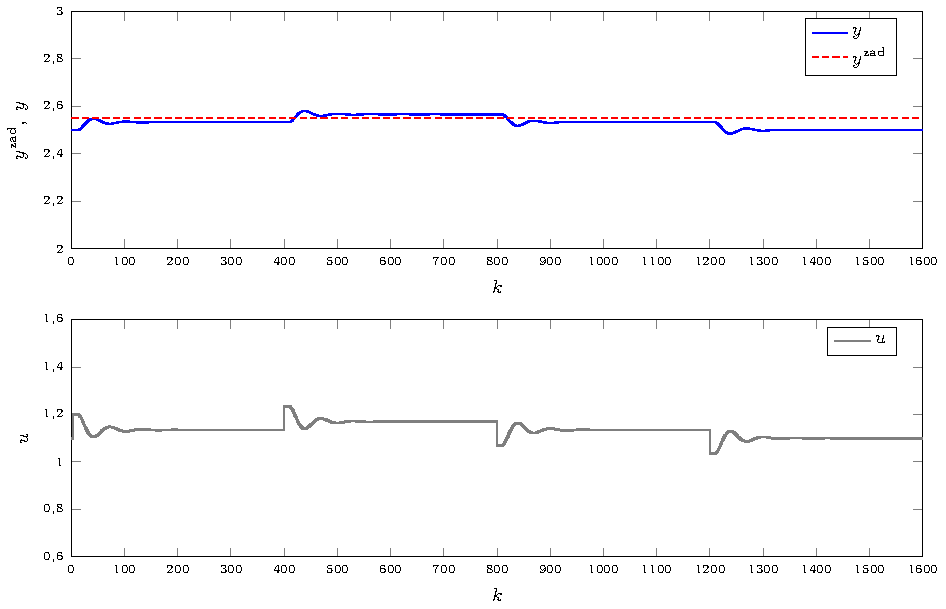
\includegraphics[scale=1]{rysunki/zapisz_pdf/PID_K=1.975_Ti=Inf_Td=0.00.pdf} 
\caption{Regulator PID dla $K=\num{1.975}$, $T_{\mathrm{i}}=inf$, $T_{\mathrm{d}}=0$} 
\label{r_pgfplots_PID_K=1.975_Ti=Inf_Td=0.00} 
\end{figure}

Uchyb ustalony jest zdecydowanie z wysoki, żeby uznać regulację za zadowalającą. Dobierzemy więc teraz parametr $T_{\mathrm{i}}$ włączając tym samym człon całkujący. Powinno pomóc to zredukować uchyb ustalony. Na rysunkach 6.4 - 6.12 przedstawiono regulację dla różnych, eksperymentalnie dobieranych wartości parametru $T_{\mathrm{i}}$.

\begin{figure}[tb] 
\centering 
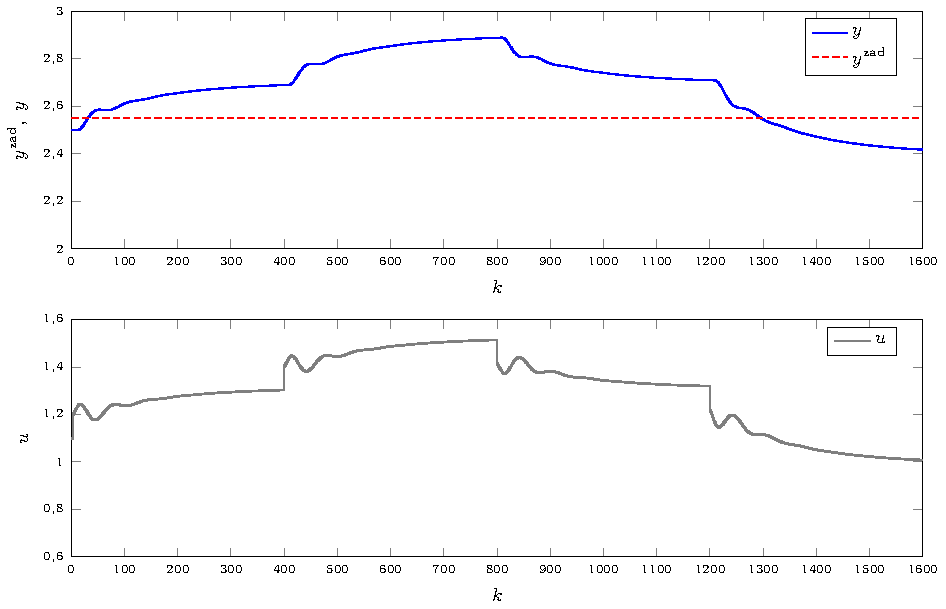
\includegraphics[scale=1]{rysunki/zapisz_pdf/PID_K=1.975_Ti=100.00_Td=0.00.pdf} 
\caption{Regulator PID dla $K=\num{1.975}$, $T_{\mathrm{i}}=100$, $T_{\mathrm{d}}=0$} 
\label{r_pgfplots_PID_K=1.975_Ti=100.00_Td=0.00} 
\end{figure}

\begin{figure}[tb] 
\centering 
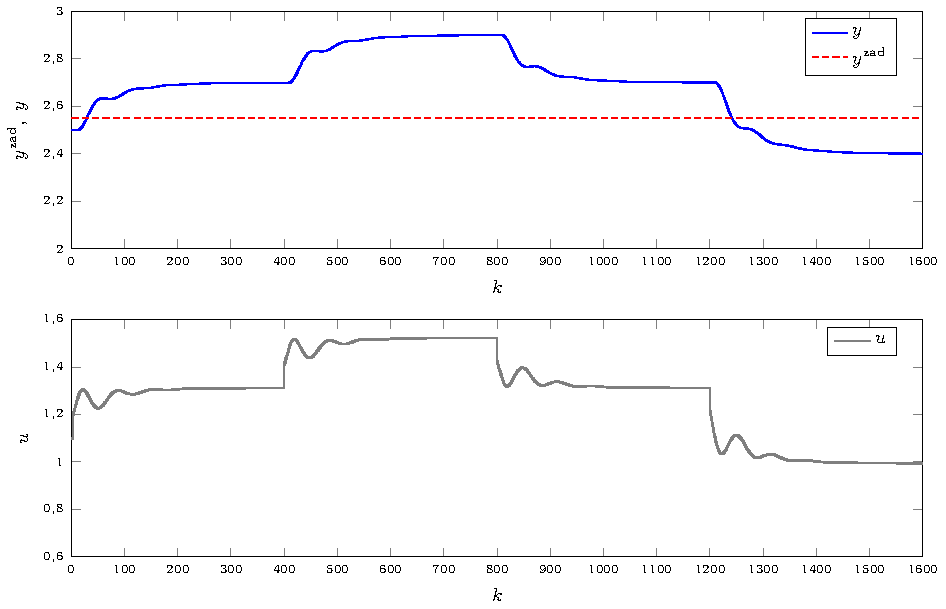
\includegraphics[scale=1]{rysunki/zapisz_pdf/PID_K=1.975_Ti=50.00_Td=0.00.pdf} 
\caption{Regulator PID dla $K=\num{1.975}$, $T_{\mathrm{i}}=50$, $T_{\mathrm{d}}=0$} 
\label{r_pgfplots_PID_K=1.975_Ti=50.00_Td=0.00} 
\end{figure}

\begin{figure}[tb] 
\centering 
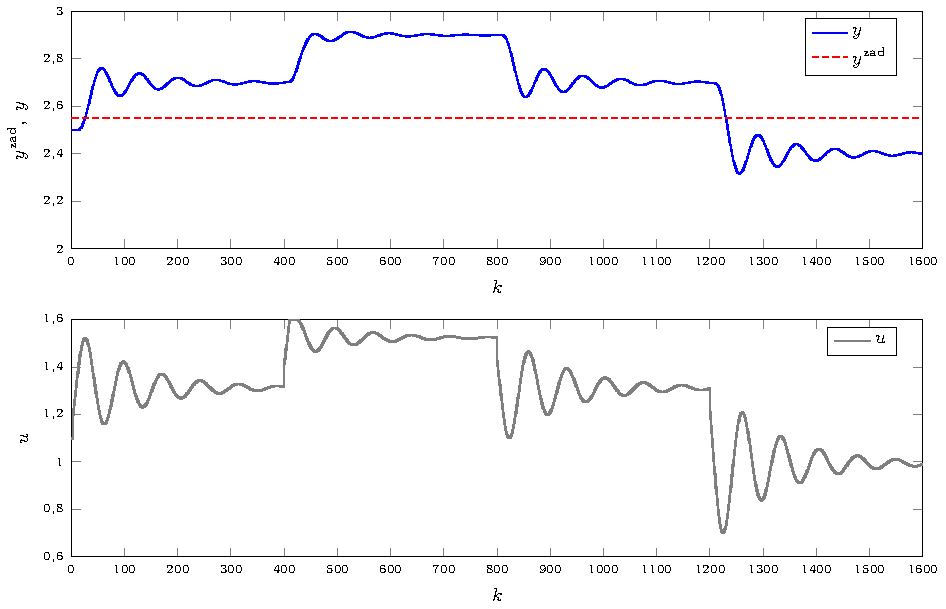
\includegraphics[scale=1]{rysunki/zapisz_pdf/PID_K=1.975_Ti=20.00_Td=0.00.pdf} 
\caption{Regulator PID dla $K=\num{1.975}$, $T_{\mathrm{i}}=20$, $T_{\mathrm{d}}=0$} 
\label{r_pgfplots_PID_K=1.975_Ti=20.00_Td=0.00} 
\end{figure}

\begin{figure}[tb] 
\centering 
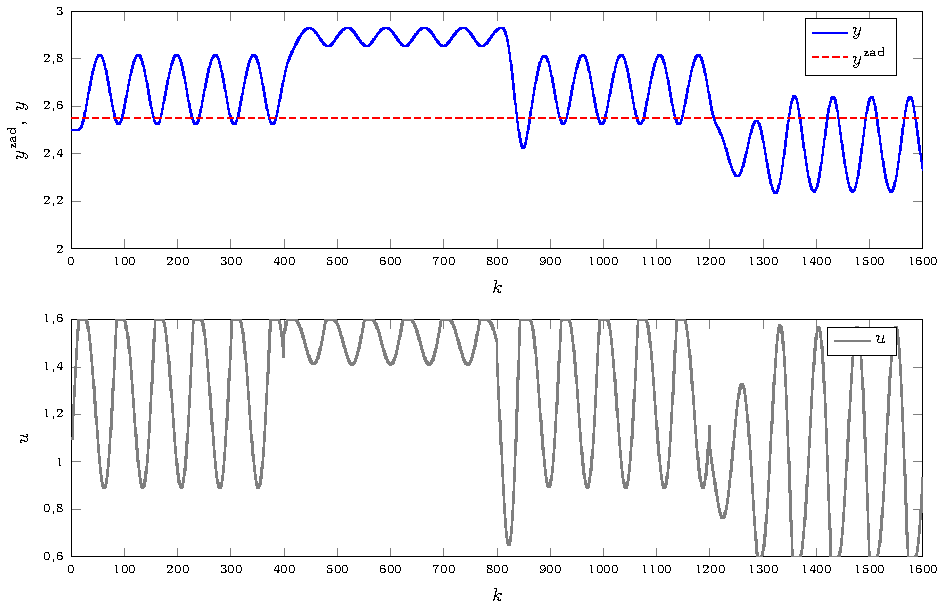
\includegraphics[scale=1]{rysunki/zapisz_pdf/PID_K=1.975_Ti=10.00_Td=0.00.pdf} 
\caption{Regulator PID dla $K=\num{1.975}$, $T_{\mathrm{i}}=10$, $T_{\mathrm{d}}=0$} 
\label{r_pgfplots_PID_K=1.975_Ti=10.00_Td=0.00} 
\end{figure}

\begin{figure}[tb] 
\centering 
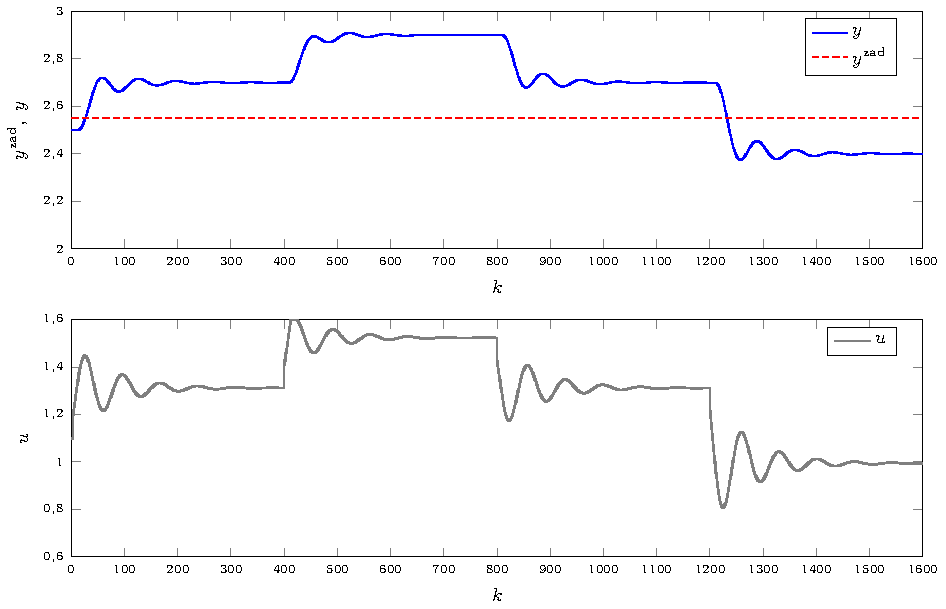
\includegraphics[scale=1]{rysunki/zapisz_pdf/PID_K=1.975_Ti=25.00_Td=0.00.pdf} 
\caption{Regulator PID dla $K=\num{1.975}$, $T_{\mathrm{i}}=25$, $T_{\mathrm{d}}=0$} 
\label{r_pgfplots_PID_K=1.975_Ti=25.00_Td=0.00} 
\end{figure}

\begin{figure}[tb] 
\centering 
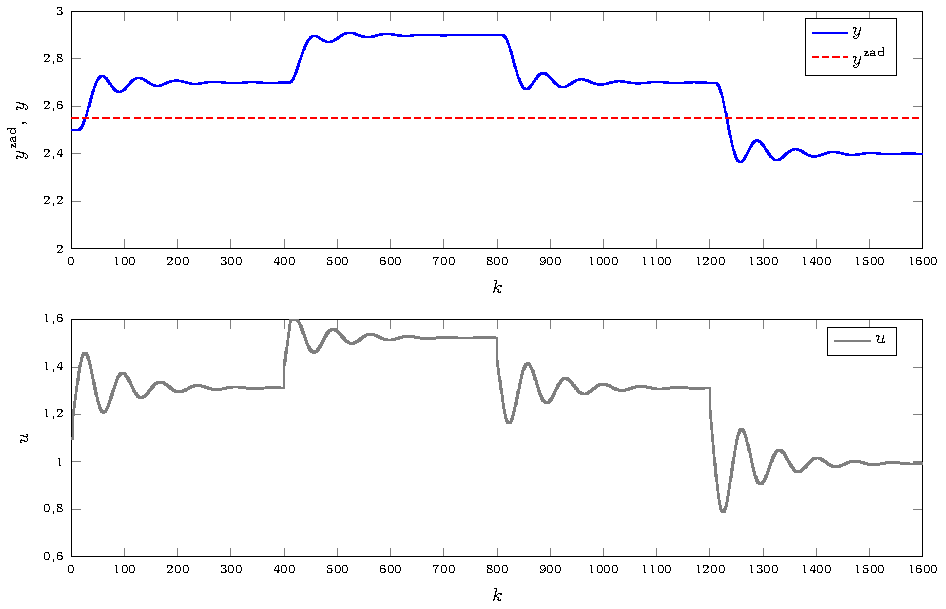
\includegraphics[scale=1]{rysunki/zapisz_pdf/PID_K=1.975_Ti=24.00_Td=0.00.pdf} 
\caption{Regulator PID dla $K=\num{1.975}$, $T_{\mathrm{i}}=24$, $T_{\mathrm{d}}=0$} 
\label{r_pgfplots_PID_K=1.975_Ti=24.00_Td=0.00} 
\end{figure}

\begin{figure}[tb] 
\centering 
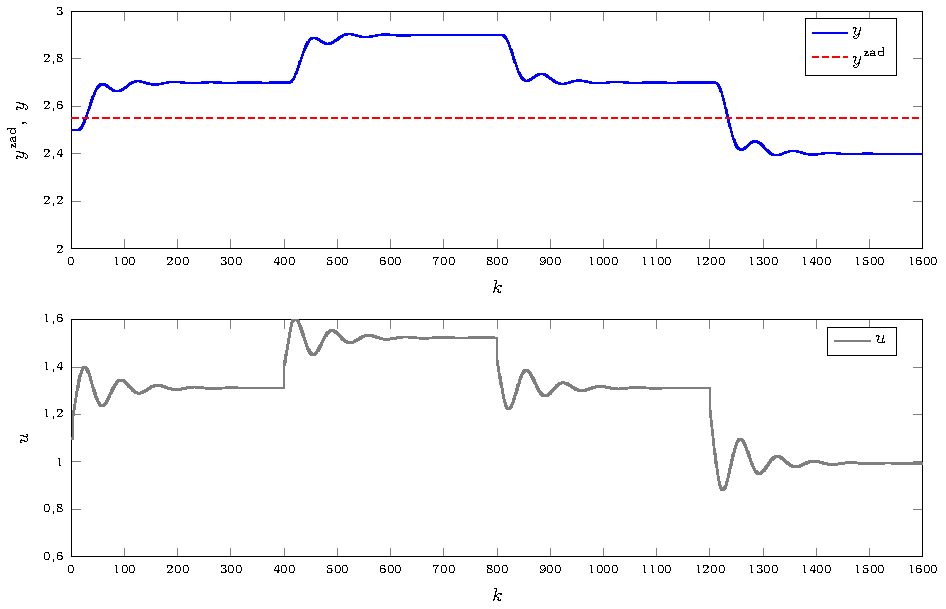
\includegraphics[scale=1]{rysunki/zapisz_pdf/PID_K=1.975_Ti=30.00_Td=0.00.pdf} 
\caption{Regulator PID dla $K=\num{1.975}$, $T_{\mathrm{i}}=30$, $T_{\mathrm{d}}=0$} 
\label{r_pgfplots_PID_K=1.975_Ti=30.00_Td=0.00} 
\end{figure}

\begin{figure}[tb] 
\centering 
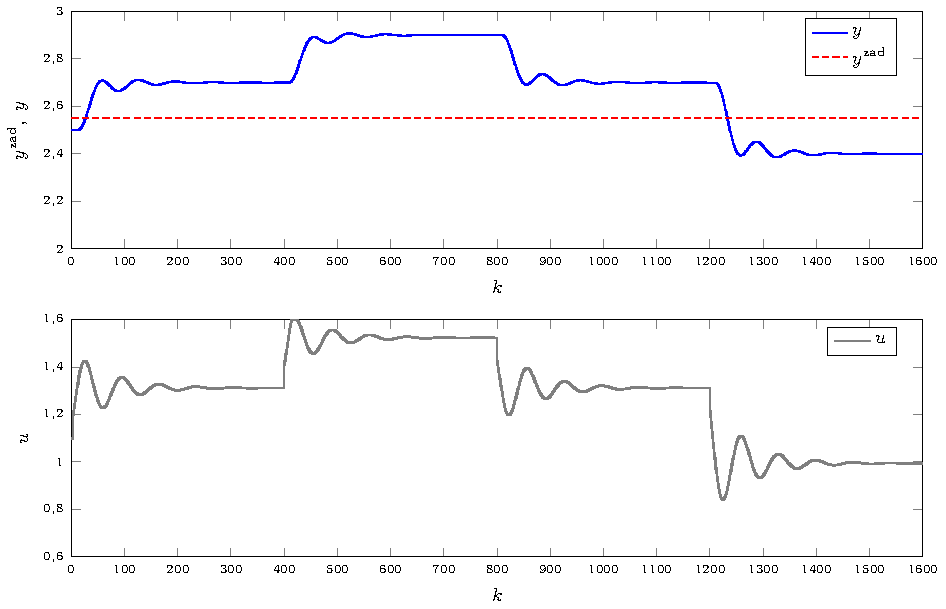
\includegraphics[scale=1]{rysunki/zapisz_pdf/PID_K=1.975_Ti=27.00_Td=0.00.pdf} 
\caption{Regulator PID dla $K=\num{1.975}$, $T_{\mathrm{i}}=27$, $T_{\mathrm{d}}=0$} 
\label{r_pgfplots_PID_K=1.975_Ti=27.00_Td=0.00} 
\end{figure}

\begin{figure}[tb] 
\centering 
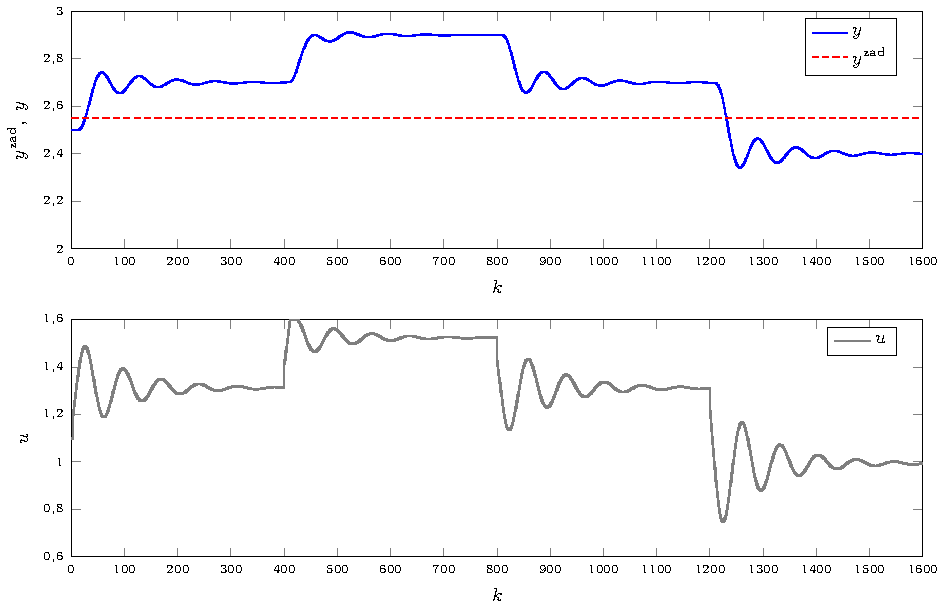
\includegraphics[scale=1]{rysunki/zapisz_pdf/PID_K=1.975_Ti=22.00_Td=0.00.pdf} 
\caption{Regulator PID dla $K=\num{1.975}$, $T_{\mathrm{i}}=22$, $T_{\mathrm{d}}=0$} 
\label{r_pgfplots_PID_K=1.975_Ti=22.00_Td=0.00} 
\end{figure}


\begin{table}
	[b] \caption{Porównanie wielkości błędu $E$ dla różnych wartości parametru $T_{\mathrm{i}}$ i dla parametru $K=\num{1.975}$}
	\label{t_T_i}
	\centering
	\sisetup{table-auto-round=true}
	\begin{small}
		\begin{tabular}{|c|c|}
			\hline
			$T_{\mathrm{i}}$	&	$E$	\\
			$inf$	&	$\num{71.3457}$		\\
			$100$ 	&	$\num{13.9366}$		\\
			$50$	&	$\num{7.8122}$		\\
			$30$	&	$\num{5.8606}$		\\
			$27$	&	$\num{5.6896}$		\\
			$25$	&	$\num{5.6210}$		\\
			$24$	&	$\num{5.6081}$		\\
			$22$	&	$\num{5.6506}$		\\
			$20$	&	$\num{5,8522}$		\\
			$10$	&	$\num{18.3320}$		\\
			\hline
			\end{tabular}
	\end{small}
\end{table}

Widzimiy, że najmniejszy błąd $E$ wystąpił dla $T_{/mathrm{i}}=24$ . Warto też zauważyć, że dla mniejszych wartości $T_{\mathrm{i}}$ zaczęły występować wolno gasnące oscylacje wartości wyjściowej. Jak widać jednak na Rys 6.9, oscylacje te są na tyle małe i gasną wystarczająco szybko, że można je tolerować. Następnym krokiem jest dobranie parametru $T_{\mathrm{d}}$. Dobierany był dla parametru $K=\num{1.975}$ i parametru $T_{\mathrm{i}}=24$.

\begin{figure}[tb] 
\centering 
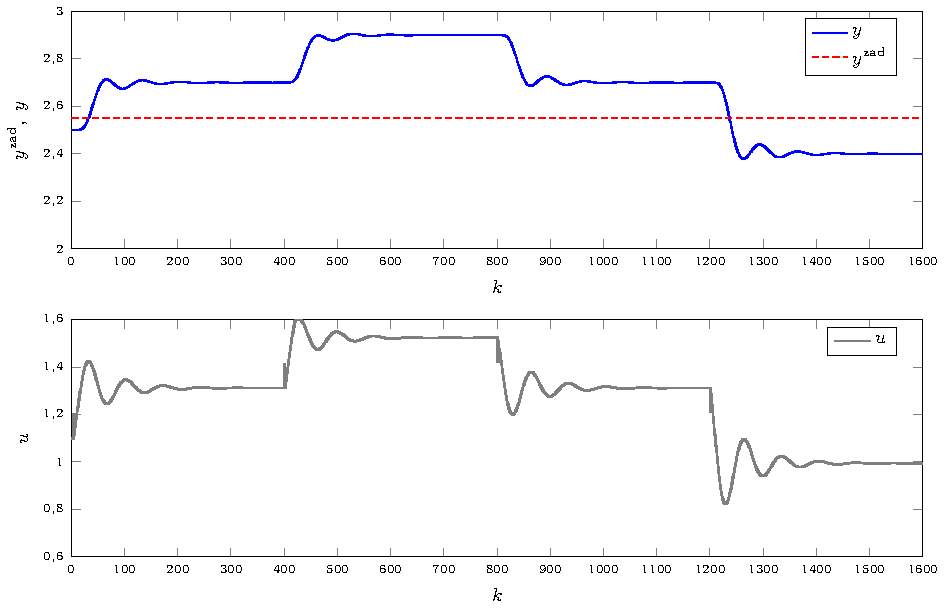
\includegraphics[scale=1]{rysunki/zapisz_pdf/PID_K=1.975_Ti=24.00_Td=1.00.pdf} 
\caption{Regulator PID dla $K=\num{1.975}$, $T_{\mathrm{i}}=24$, $T_{\mathrm{d}}=1$} 
\label{r_pgfplots_PID_K=1.975_Ti=24.00_Td=1.00} 
\end{figure}

\begin{figure}[tb] 
\centering 
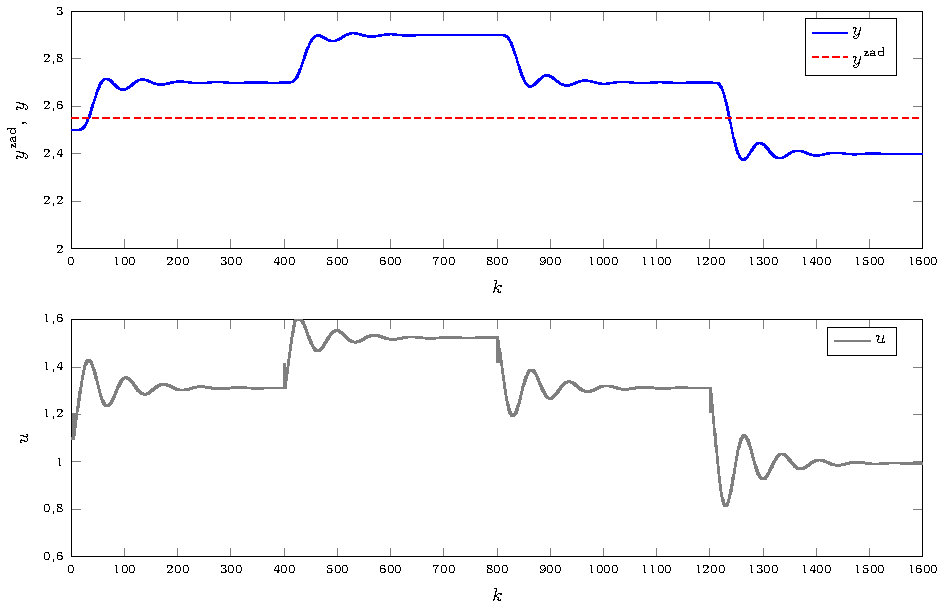
\includegraphics[scale=1]{rysunki/zapisz_pdf/PID_K=1.975_Ti=24.00_Td=0.50.pdf} 
\caption{Regulator PID dla $K=\num{1.975}$, $T_{\mathrm{i}}=24$, $T_{\mathrm{d}}=\num{0.5}$} 
\label{r_pgfplots_PID_K=1.975_Ti=24.00_Td=0.50} 
\end{figure}

\begin{figure}[tb] 
\centering 
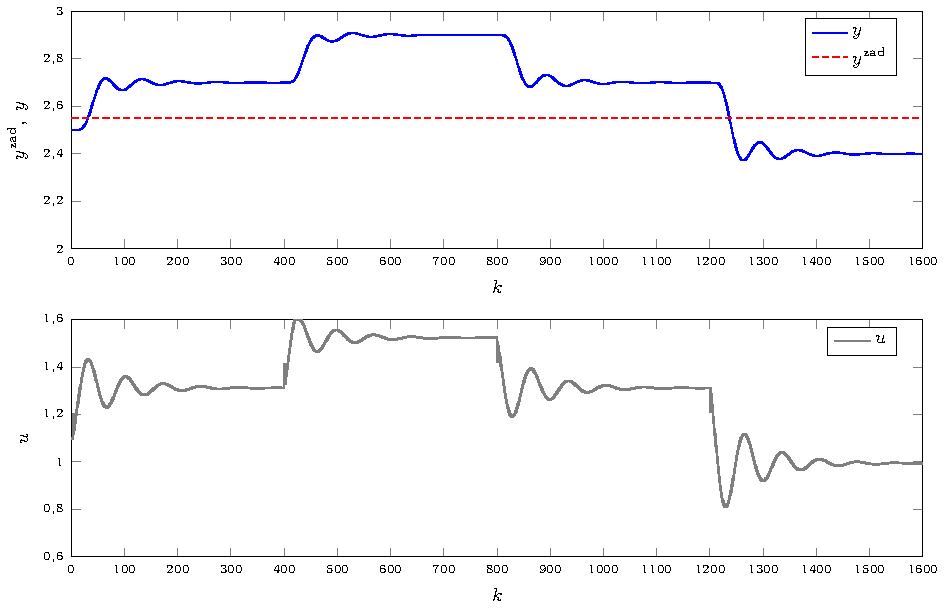
\includegraphics[scale=1]{rysunki/zapisz_pdf/PID_K=1.975_Ti=24.00_Td=0.25.pdf} 
\caption{Regulator PID dla $K=\num{1.975}$, $T_{\mathrm{i}}=24$, $T_{\mathrm{d}}=\num{0.25}$} 
\label{r_pgfplots_PID_K=1.975_Ti=24.00_Td=0.25} 
\end{figure}

\begin{figure}[tb] 
\centering 
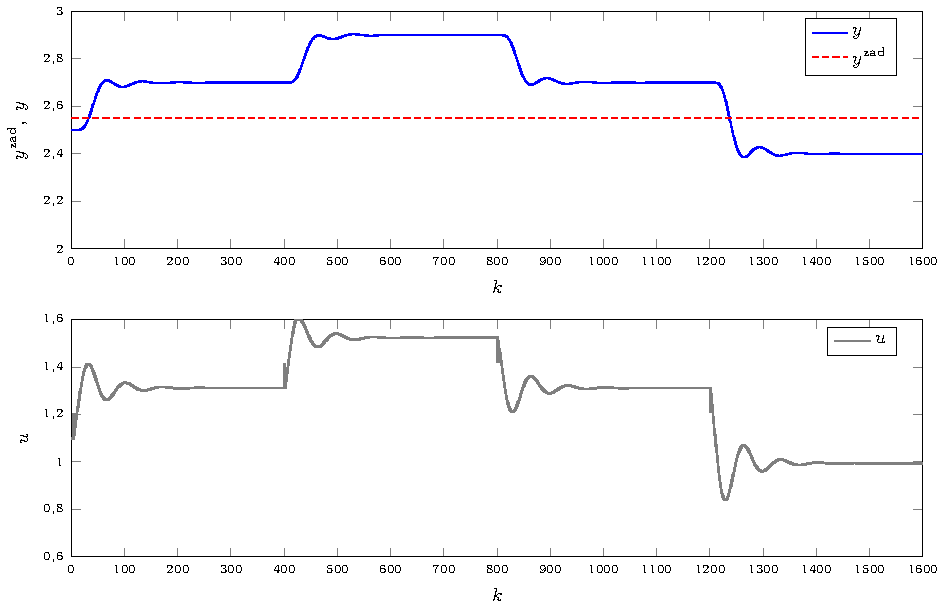
\includegraphics[scale=1]{rysunki/zapisz_pdf/PID_K=1.975_Ti=24.00_Td=2.00.pdf} 
\caption{Regulator PID dla $K=\num{1.975}$, $T_{\mathrm{i}}=24$, $T_{\mathrm{d}}=2$} 
\label{r_pgfplots_PID_K=1.975_Ti=24.00_Td=2.00} 
\end{figure}

\begin{figure}[tb] 
\centering 
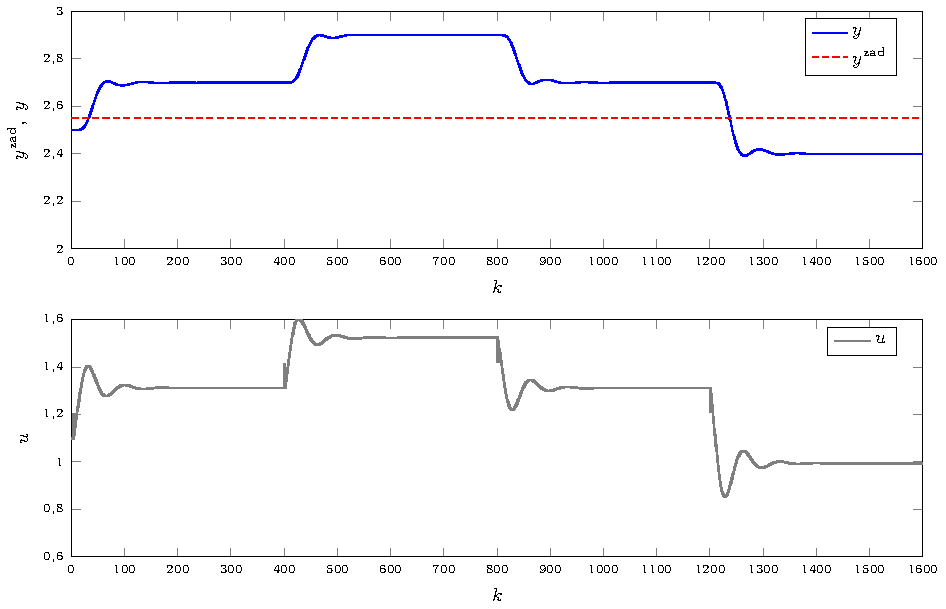
\includegraphics[scale=1]{rysunki/zapisz_pdf/PID_K=1.975_Ti=24.00_Td=3.00.pdf} 
\caption{Regulator PID dla $K=\num{1.975}$, $T_{\mathrm{i}}=24$, $T_{\mathrm{d}}=3$} 
\label{r_pgfplots_PID_K=1.975_Ti=24.00_Td=3.00} 
\end{figure}

\begin{figure}[tb] 
\centering 
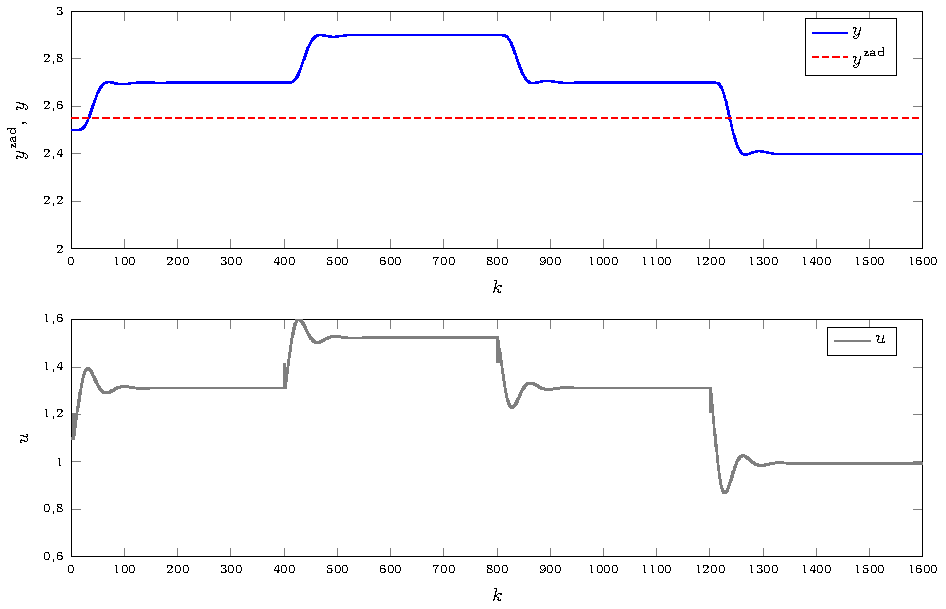
\includegraphics[scale=1]{rysunki/zapisz_pdf/PID_K=1.975_Ti=24.00_Td=4.00.pdf} 
\caption{Regulator PID dla $K=\num{1.975}$, $T_{\mathrm{i}}=24$, $T_{\mathrm{d}}=4$} 
\label{r_pgfplots_PID_K=1.975_Ti=24.00_Td=4.00} 
\end{figure}

\begin{table}
	[b] \caption{Porównanie wielkości błędu $E$ dla różnych wartości parametru $T_{\mathrm{d}}$ i dla parametru $K=1.975$ oraz parametru $T_{\mathrm{i}}=24$}
	\label{t_T_i}
	\centering
	\sisetup{table-auto-round=true}
	\begin{small}
		\begin{tabular}{|c|c|}
			\hline
			$T_{\mathrm{d}}$	&	$E$	\\
			$0$		&	$\num{5.6081}$		\\
			$\num{0.5}$ 	&	$\num{6.6090}$		\\
			$\num{0.25}	$ & $\num{6.4963}$ \\
			$1$ 	&	$\num{6.5853}$		\\
			$2$		&	$\num{6.5632}$	\\
			$3$		&	$\num{6.5644}$	\\
			$4$		&	$\num{6.5808}$	\\
			\hline
			\end{tabular}
	\end{small}
\end{table}

Jak widać z tabelki dodanie członu różniczkującego zwiększyło wartość błędu $E$. Na rysunkach widać jednak, że wystepujące wcześniej oscylacje znacznie zmniejszyły się dzięki działaniu członu, co jest pożądane, zwłaszcza dla obiektów rzeczywistych. Można dobrać różne wartości $T_{\mathrm{d}}$ w zależności od pożądanego tłumienia oscylacji, jako kompromis między tłumieniem a wskaźnikiem jakości $E$ wybrane zostało $T_{\mathrm{d}}=3$ (Rys 6.17). Ostateczne parametry PID otrzymane w wyniku eksperymentów to: $K=\num{1.975}$, $T_{\mathrm{i}}=24$, $T_{\mathrm{d}}=3$. Oczywiście nie są to pewnie idealne parametry regulatora.


\section{Eksperymentalne dobranie parametrów DMC}

Do eksperymentalnego dobrania parametrów DMC użyto nastepującej metody eksperymentalnej:
\begin{enumerate}
\item Przyjęcie maksymalnego możliwego parametry $D$, równego długości odpowiedzi skokowej aż do jej ustabilizowania, w naszym przypadku $D=200$. 
\item Dla maksymalnie dużego parametru $D$ stopniowe zmniejszanie parametrów $N$ i $N_{\mathrm{u}}$ ($N$ musi byc cały czas równe $N_{\mathrm{u}}$, aż osiągniemy zadowalające wyniki.
\item Dla tak dobranych parametrów $D$ i $N$ dobranie parametru $N_{\mathrm{u}}$ dającego zadowalające wyniki.
\end{enumerate}


Wyjściowy regulator DMC ($D=N=N_{\mathrm{u}}=200$) przeedstawiony jest na Rys 6.13. Po błędzie i ryunku widać, że już i taki regulator DMC sprawia się lepiej niż regulator PID. Ponieważ dla wartości $N\ge{50}$ regulator zachowywał się w przybliżeniu identycznie nie zamieszczone zostały wykresy dla nich.


\begin{figure}[tb] 
\centering 
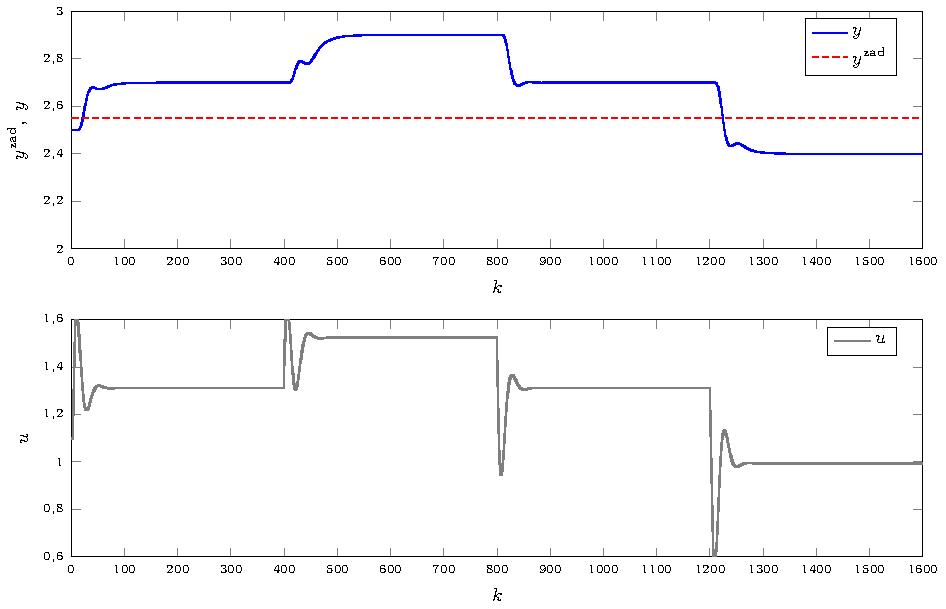
\includegraphics[scale=1]{rysunki/zapisz_pdf/DMC_D=200.000_N=200.00_Nu=200.00.pdf} 
\caption{Regulator DMC dla $D=200$, $N=200$, $N_{\mathrm{u}}=200$} 
\label{r_pgfplots_DMC_D=200.000_N=200.00_Nu=200.00} 
\end{figure}

\begin{figure}[tb] 
\centering 
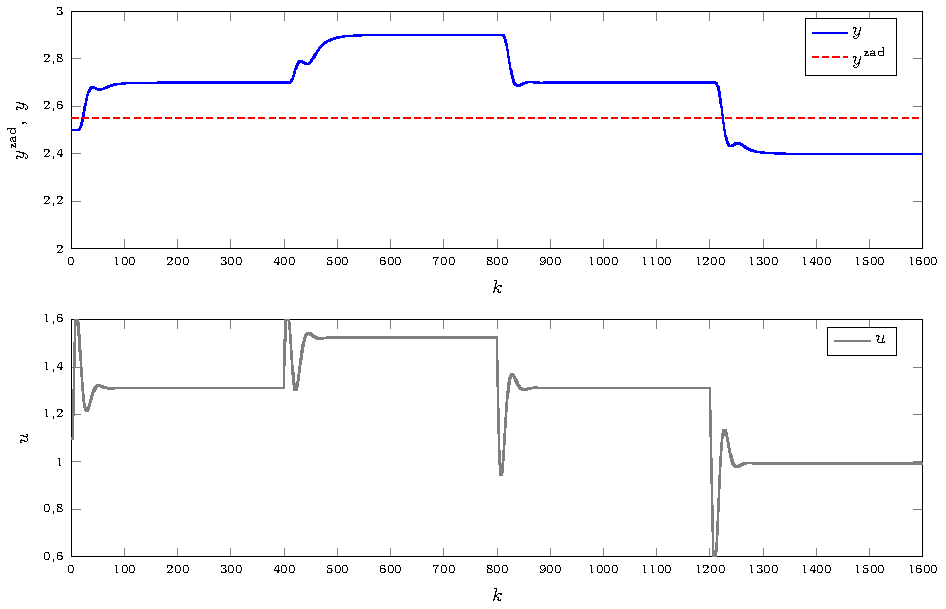
\includegraphics[scale=1]{rysunki/zapisz_pdf/DMC_D=200.000_N=40.00_Nu=40.00.pdf} 
\caption{Regulator DMC dla $D=200$, $N=40$, $N_{\mathrm{u}}=40$} 
\label{r_pgfplots_DMC_D=200.000_N=40.00_Nu=40.00} 
\end{figure}

\begin{figure}[tb] 
\centering 
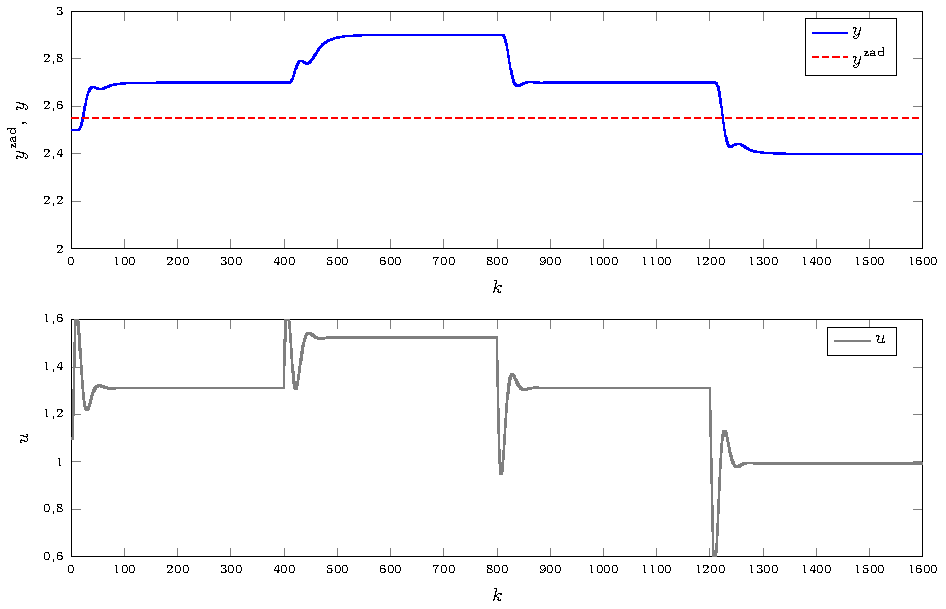
\includegraphics[scale=1]{rysunki/zapisz_pdf/DMC_D=200.000_N=30.00_Nu=30.00.pdf} 
\caption{Regulator DMC dla $D=200$, $N=30$, $N_{\mathrm{u}}=30$} 
\label{r_pgfplots_DMC_D=200.000_N=30.00_Nu=30.00} 
\end{figure}

\begin{figure}[tb] 
\centering 
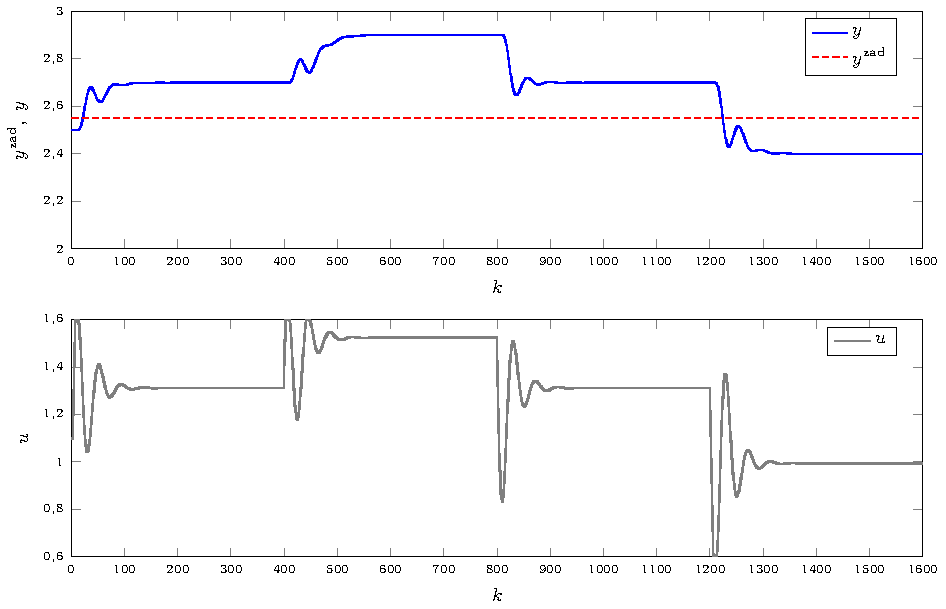
\includegraphics[scale=1]{rysunki/zapisz_pdf/DMC_D=200.000_N=20.00_Nu=20.00.pdf} 
\caption{Regulator DMC dla $D=200$, $N=20$, $N_{\mathrm{u}}=20$} 
\label{r_pgfplots_DMC_D=200.000_N=20.00_Nu=20.00} 
\end{figure}

\begin{figure}[tb] 
\centering 
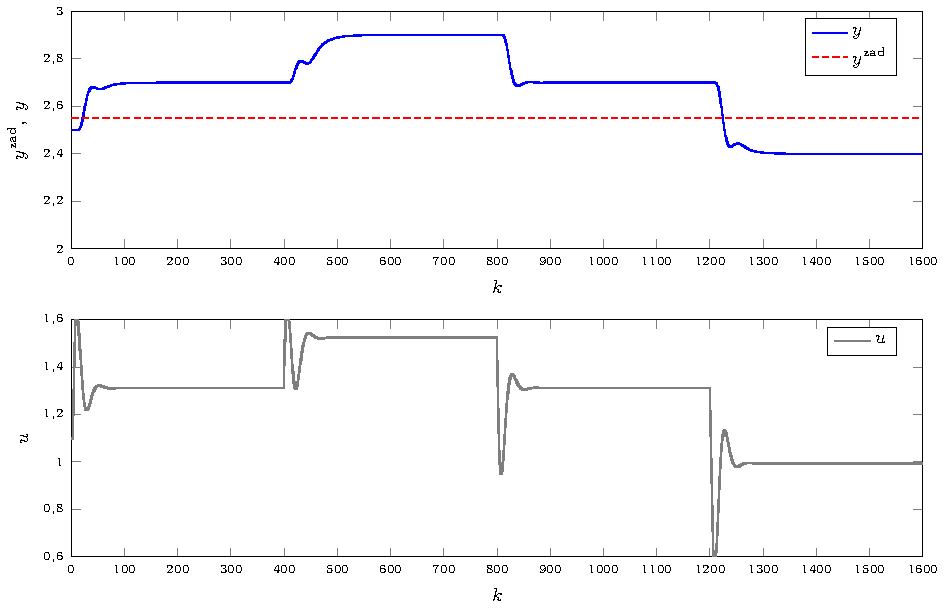
\includegraphics[scale=1]{rysunki/zapisz_pdf/DMC_D=200.000_N=35.00_Nu=35.00.pdf} 
\caption{Regulator DMC dla $D=200$, $N=35$, $N_{\mathrm{u}}=35$} 
\label{r_pgfplots_DMC_D=200.000_N=35.00_Nu=35.00} 
\end{figure}

\begin{figure}[tb] 
\centering 
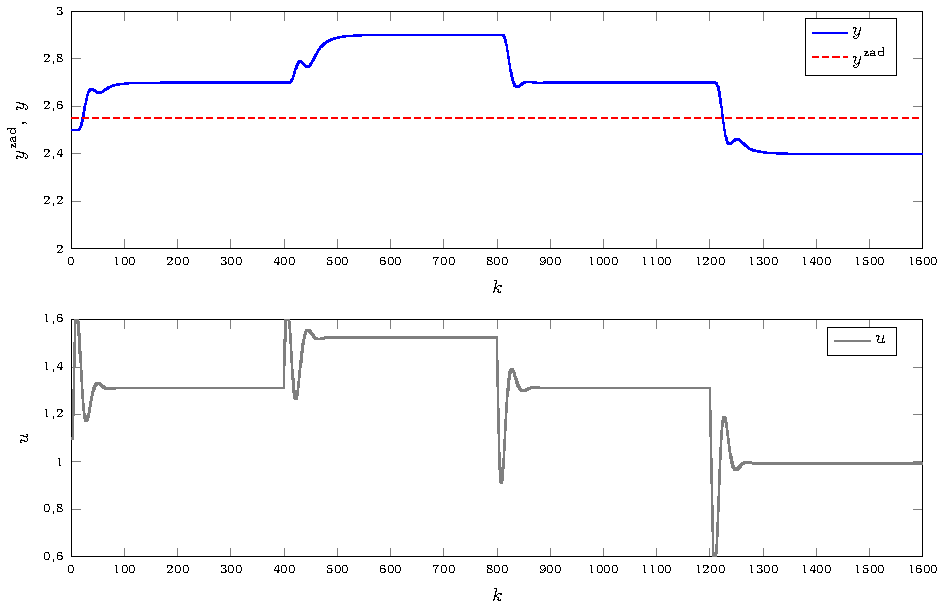
\includegraphics[scale=1]{rysunki/zapisz_pdf/DMC_D=200.000_N=25.00_Nu=25.00.pdf} 
\caption{Regulator DMC dla $D=200$, $N=25$, $N_{\mathrm{u}}=25$} 
\label{r_pgfplots_DMC_D=200.000_N=25.00_Nu=25.00} 
\end{figure}

\begin{figure}[tb] 
\centering 
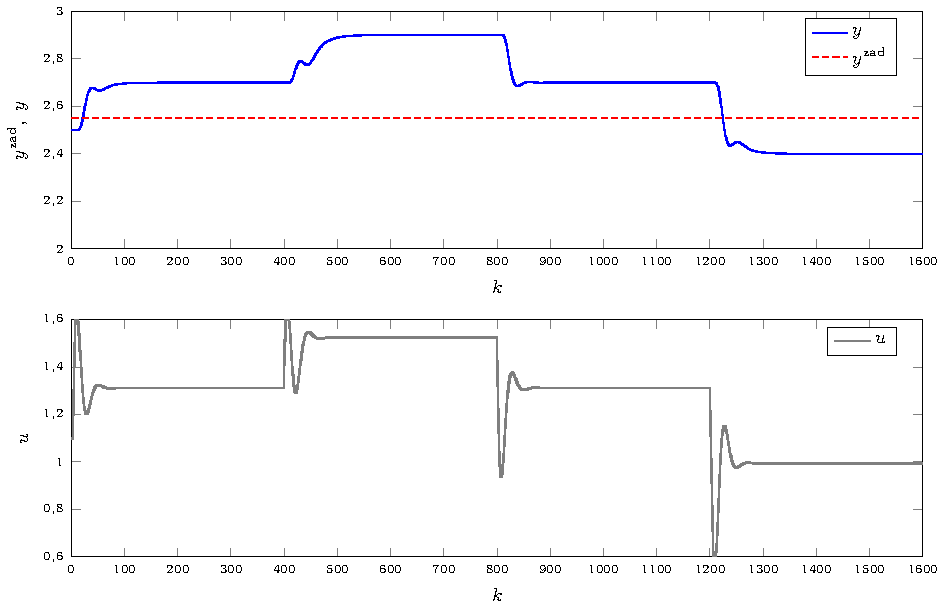
\includegraphics[scale=1]{rysunki/zapisz_pdf/DMC_D=200.000_N=27.00_Nu=27.00.pdf} 
\caption{Regulator DMC dla $D=200$, $N=27$, $N_{\mathrm{u}}=27$} 
\label{r_pgfplots_DMC_D=200.000_N=27.00_Nu=27.00} 
\end{figure}

\begin{figure}[tb] 
\centering 
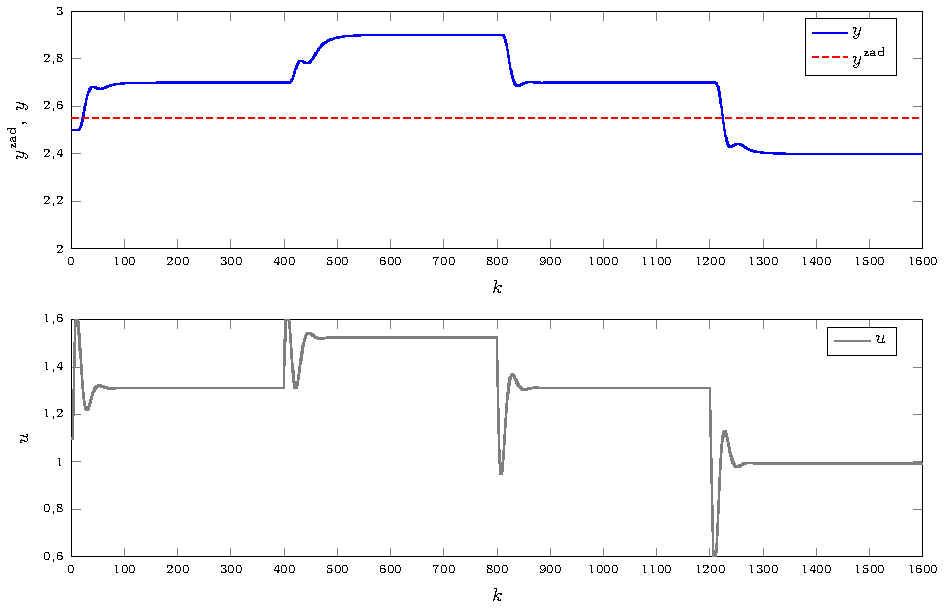
\includegraphics[scale=1]{rysunki/zapisz_pdf/DMC_D=200.000_N=32.00_Nu=32.00.pdf} 
\caption{Regulator DMC dla $D=200$, $N=32$, $N_{\mathrm{u}}=32$} 
\label{r_pgfplots_DMC_D=200.000_N=32.00_Nu=32.00} 
\end{figure}

\begin{table}
	[b] \caption{Porównanie wielkości błędu $E$ dla różnych wartości parametrów $N$ i $N_{\mathrm{u}}$ i dla parametru $D=200$}
	\label{t_T_i}
	\centering
	\sisetup{table-auto-round=true}
	\begin{small}
		\begin{tabular}{|c|c|}
			\hline
			$N$ i $N_{\mathrm{u}}$	&	$E$	\\
			$200$	&	$\num{4.8557}$		\\
			$150$ 	&	$\num{4.8557}$		\\
			$100$ 	&	$\num{4.8557}$ 		\\
			$50$ 	&	$\num{4.8556}$		\\
			$40$	&	$\num{4.8571}$	\\
			$35$	&	$\num{4.8403}$	\\
			$30$	&	$\num{4.8356}$	\\
			$32$	&	$\num{4.8301}$	\\
			$27$	&	$\num{4.8876}$	\\
			$25$	&	$\num{4.9796}$	\\
			$20$	&	$\num{5.3776}$	\\
			\hline
			\end{tabular}
	\end{small}
\end{table}

Większość przebiegów zapewnia zadowalający kształt funkcji wyjściowej, dlatego wybierając najlepszą wartość parametru $N$ kierować będziemy się wartością wskaźnika jakości $E$, co sprawia, że najlepszą regulację otrzymujemy dla $N=N_{\mathrm{u}}=32$. Wartość parametru $N_{\mathrm{u}}$ dobierana więc będzie dla $D=200$ i $N=32$. Ponieważ dla wartości $N_{\mathrm{u}}\ge{18}$ regulator zachowywał się w przybliżeniu identycznie nie zamieszczone zostały wykresy dla nich.

\begin{figure}[tb] 
\centering 
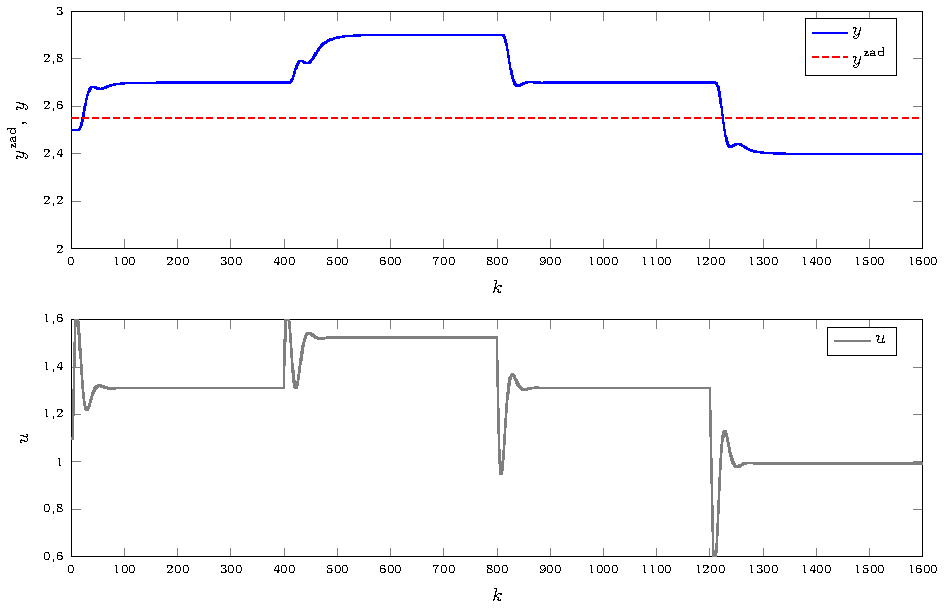
\includegraphics[scale=1]{rysunki/zapisz_pdf/DMC_D=200.000_N=32.00_Nu=15.00.pdf} 
\caption{Regulator DMC dla $D=200$, $N=32$, $N_{\mathrm{u}}=15$} 
\label{r_pgfplots_DMC_D=200.000_N=32.00_Nu=15.00} 
\end{figure}

\begin{figure}[tb] 
\centering 
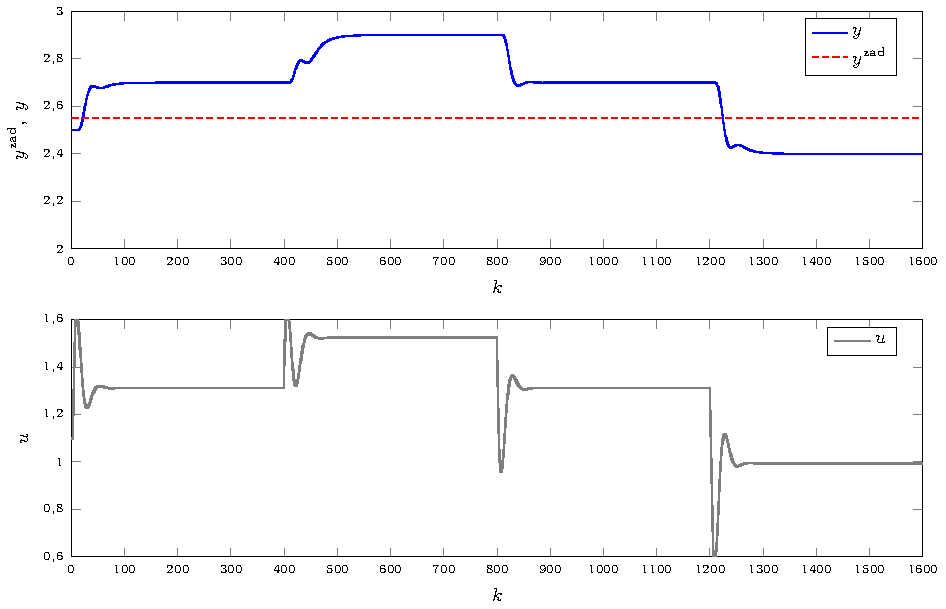
\includegraphics[scale=1]{rysunki/zapisz_pdf/DMC_D=200.000_N=32.00_Nu=10.00.pdf} 
\caption{Regulator DMC dla $D=200$, $N=32$, $N_{\mathrm{u}}=10$} 
\label{r_pgfplots_DMC_D=200.000_N=32.00_Nu=10.00} 
\end{figure}

\begin{figure}[tb] 
\centering 
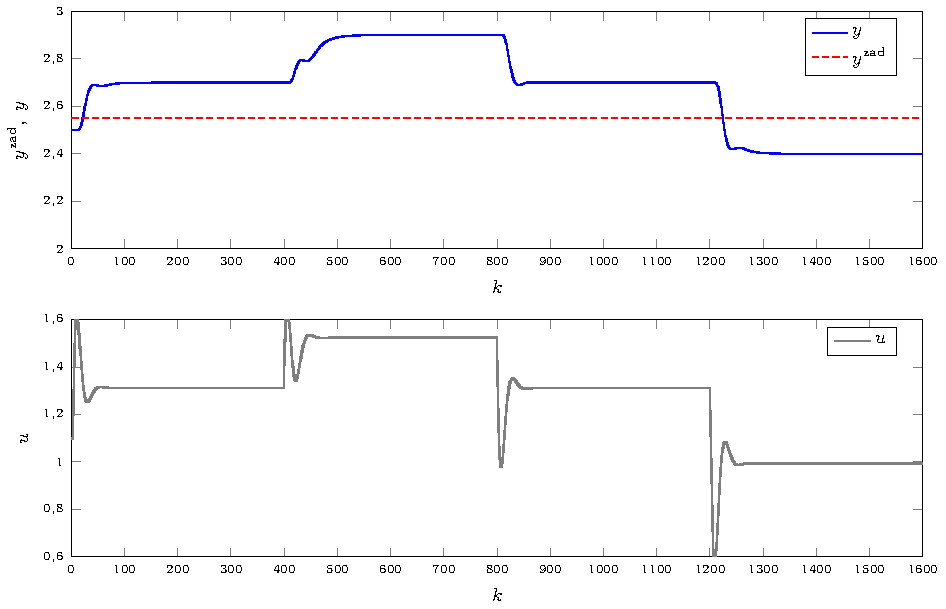
\includegraphics[scale=1]{rysunki/zapisz_pdf/DMC_D=200.000_N=32.00_Nu=7.00.pdf} 
\caption{Regulator DMC dla $D=200$, $N=32$, $N_{\mathrm{u}}=7$} 
\label{r_pgfplots_DMC_D=200.000_N=32.00_Nu=7.00} 
\end{figure}

\begin{figure}[tb] 
\centering 
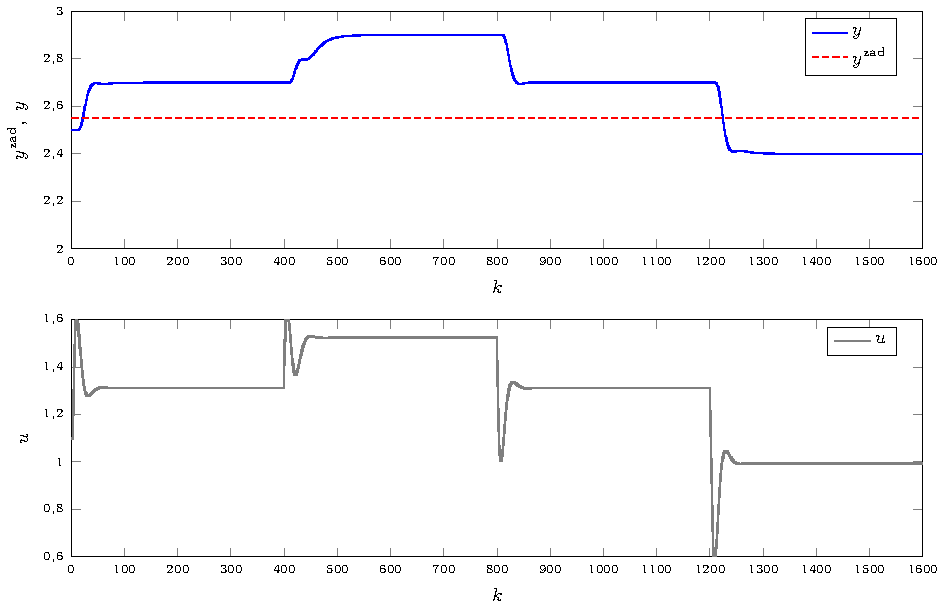
\includegraphics[scale=1]{rysunki/zapisz_pdf/DMC_D=200.000_N=32.00_Nu=5.00.pdf} 
\caption{Regulator DMC dla $D=200$, $N=32$, $N_{\mathrm{u}}=5$} 
\label{r_pgfplots_DMC_D=200.000_N=32.00_Nu=5.00} 
\end{figure}

\begin{figure}[tb] 
\centering 
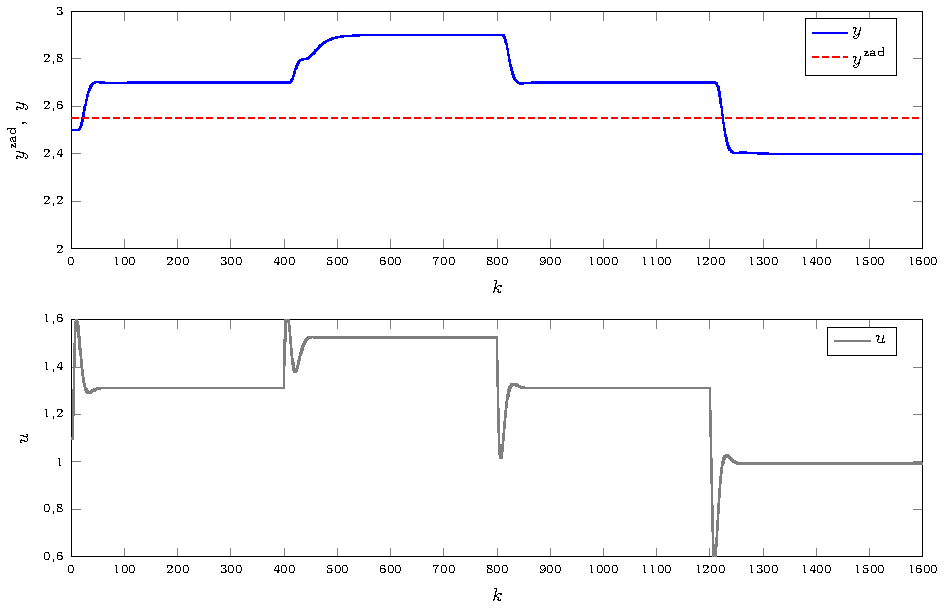
\includegraphics[scale=1]{rysunki/zapisz_pdf/DMC_D=200.000_N=32.00_Nu=4.00.pdf} 
\caption{Regulator DMC dla $D=200$, $N=32$, $N_{\mathrm{u}}=4$} 
\label{r_pgfplots_DMC_D=200.000_N=32.00_Nu=4.00} 
\end{figure}

\begin{figure}[tb] 
\centering 
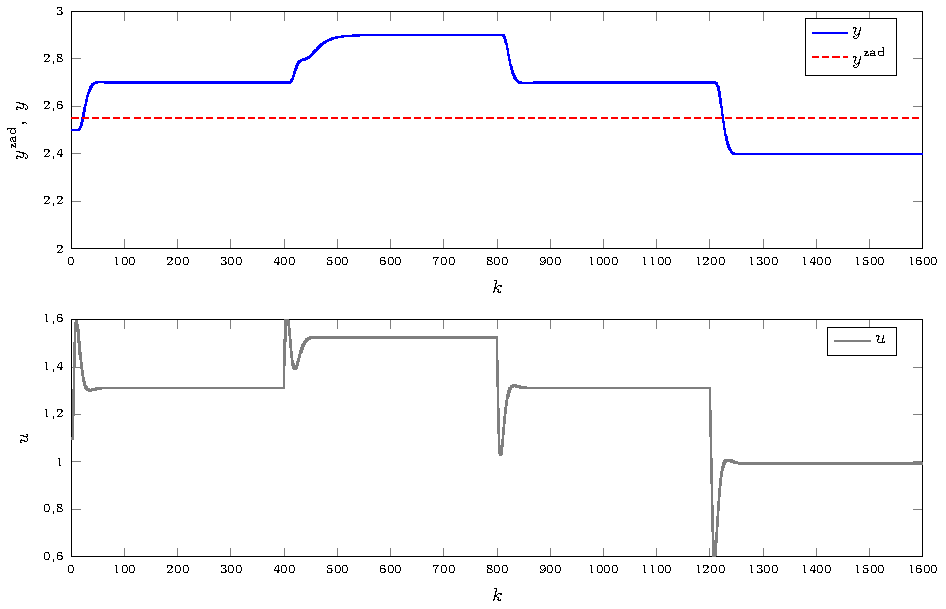
\includegraphics[scale=1]{rysunki/zapisz_pdf/DMC_D=200.000_N=32.00_Nu=3.00.pdf} 
\caption{Regulator DMC dla $D=200$, $N=32$, $N_{\mathrm{u}}=3$} 
\label{r_pgfplots_DMC_D=200.000_N=32.00_Nu=3.00} 
\end{figure}


\begin{table}
	[b] \caption{Porównanie wielkości błędu $E$ dla różnych wartości parametru $N_{\mathrm{u}}$ i dla parametrów $D=200$ i $N=32$}
	\label{t_T_i}
	\centering
	\sisetup{table-auto-round=true}
	\begin{small}
		\begin{tabular}{|c|c|}
			\hline
			$N_{\mathrm{u}}$	&	$E$	\\
			$32$	&	$\num{4.8301}$		\\
			$25$ 	&	$\num{4.8301}$		\\
			$20$ 	&	$\num{4.8301}$ 		\\
			$18$ 	&	$\num{4.8301}$		\\
			$15$	&	$\num{4.8288}$	\\
			$10$	&	$\num{4.8027}$	\\
			$7$		&	$\num{4.7471}$	\\
			$5$		&	$\num{4.7036}$	\\
			$4$		&	$\num{4.6905}$	\\
			$3$		&	$\num{4.7039}$	\\
			\hline
			\end{tabular}
	\end{small}
\end{table}


Dla różnych wartości parametru $N_{\mathrm{u}}$ przebiegi są w większości podobne, jedynie wartość wskaźnika jakości $E$ różni się nieznacznie między nimi. Z tego powodu, wybrany zostanie regulator o parametrach $D=200$, $N=32$ i $N_{\mathrm{u}}=4$ (Rys 6.31).
